\documentclass[portrait,final,paperwidth=90cm,paperheight=130cm,fontscale=0.295]{baposter}
\usepackage{color, colortbl}
\usepackage[backend=bibtex]{biblatex}
\usepackage{float}
% \usepackage{subfigure}
% \usepackage{chngcntr}
% \usepackage{cite}
\usepackage{wrapfig}
% \usepackage{subcaption}
\usepackage[font=small,labelfont=bf]{caption}
\usepackage{subcaption}
\usepackage[export]{adjustbox}
\usepackage{calc}
\usepackage{graphicx}
\usepackage{amsmath}
\usepackage{amssymb}
% \usepackage{relsize}
\usepackage{multirow}
\usepackage{rotating}
\usepackage{bm}
\usepackage{url}
\usepackage{multicol}

%\usepackage{times}
%\usepackage{helvet}
%\usepackage{bookman}
\usepackage{palatino}
{\footnotesize
\bibliography{biblio,linkers,arquitectura}}
% \newcommand{\captionfont}{\footnotesize}
\definecolor{Gray}{gray}{0.9}
\definecolor{GrayOscuro}{gray}{0.71}
\definecolor{celestito}{rgb}{0.88,1,1}

\graphicspath{{images/}{../images/}}
\usetikzlibrary{calc}

\newcommand{\SET}[1]  {\ensuremath{\mathcal{#1}}}
\newcommand{\MAT}[1]  {\ensuremath{\boldsymbol{#1}}}
\newcommand{\VEC}[1]  {\ensuremath{\boldsymbol{#1}}}
\newcommand{\Video}{\SET{V}}
\newcommand{\video}{\VEC{f}}
\newcommand{\track}{x}
\newcommand{\Track}{\SET T}
\newcommand{\LMs}{\SET L}
\newcommand{\lm}{l}
\newcommand{\PosE}{\SET P}
\newcommand{\posE}{\VEC p}
\newcommand{\negE}{\VEC n}
\newcommand{\NegE}{\SET N}
\newcommand{\Occluded}{\SET O}
\newcommand{\occluded}{o}

%%%%%%%%%%%%%%%%%%%%%%%%%%%%%%%%%%%%%%%%%%%%%%%%%%%%%%%%%%%%%%%%%%%%%%%%%%%%%%%%
%%%% Some math symbols used in the text
%%%%%%%%%%%%%%%%%%%%%%%%%%%%%%%%%%%%%%%%%%%%%%%%%%%%%%%%%%%%%%%%%%%%%%%%%%%%%%%%

%%%%%%%%%%%%%%%%%%%%%%%%%%%%%%%%%%%%%%%%%%%%%%%%%%%%%%%%%%%%%%%%%%%%%%%%%%%%%%%%
% Multicol Settings
%%%%%%%%%%%%%%%%%%%%%%%%%%%%%%%%%%%%%%%%%%%%%%%%%%%%%%%%%%%%%%%%%%%%%%%%%%%%%%%%
\setlength{\columnsep}{1.5em}
\setlength{\columnseprule}{0mm}

%%%%%%%%%%%%%%%%%%%%%%%%%%%%%%%%%%%%%%%%%%%%%%%%%%%%%%%%%%%%%%%%%%%%%%%%%%%%%%%%
% Save space in lists. Use this after the opening of the list
%%%%%%%%%%%%%%%%%%%%%%%%%%%%%%%%%%%%%%%%%%%%%%%%%%%%%%%%%%%%%%%%%%%%%%%%%%%%%%%%
\newcommand{\compresslist}{%
\setlength{\itemsep}{1pt}%
\setlength{\parskip}{0pt}%
\setlength{\parsep}{0pt}%
}

%%%%%%%%%%%%%%%%%%%%%%%%%%%%%%%%%%%%%%%%%%%%%%%%%%%%%%%%%%%%%%%%%%%%%%%%%%%%%%
%%% Begin of Document
%%%%%%%%%%%%%%%%%%%%%%%%%%%%%%%%%%%%%%%%%%%%%%%%%%%%%%%%%%%%%%%%%%%%%%%%%%%%%%

\begin{document}

%%%%%%%%%%%%%%%%%%%%%%%%%%%%%%%%%%%%%%%%%%%%%%%%%%%%%%%%%%%%%%%%%%%%%%%%%%%%%%
%%% Here starts the poster
%%%---------------------------------------------------------------------------
%%% Format it to your taste with the options
%%%%%%%%%%%%%%%%%%%%%%%%%%%%%%%%%%%%%%%%%%%%%%%%%%%%%%%%%%%%%%%%%%%%%%%%%%%%%%
% Define some colors

%\definecolor{lightblue}{cmyk}{0.83,0.24,0,0.12}
\definecolor{lightblue}{rgb}{0.145,0.6666,1}

% Draw a video
\newlength{\FSZ}
\newcommand{\drawvideo}[3]{% [0 0.25 0.5 0.75 1 1.25 1.5]
   \noindent\pgfmathsetlength{\FSZ}{\linewidth/#2}
   \begin{tikzpicture}[outer sep=0pt,inner sep=0pt,x=\FSZ,y=\FSZ]
   \draw[color=lightblue!50!black] (0,0) node[outer sep=0pt,inner sep=0pt,text width=\linewidth,minimum height=0] (video) {\noindent#3};
   \path [fill=lightblue!50!black,line width=0pt] 
     (video.north west) rectangle ([yshift=\FSZ] video.north east) 
    \foreach \x in {1,2,...,#2} {
      {[rounded corners=0.6] ($(video.north west)+(-0.7,0.8)+(\x,0)$) rectangle +(0.4,-0.6)}
    }
;
   \path [fill=lightblue!50!black,line width=0pt] 
     ([yshift=-1\FSZ] video.south west) rectangle (video.south east) 
    \foreach \x in {1,2,...,#2} {
      {[rounded corners=0.6] ($(video.south west)+(-0.7,-0.2)+(\x,0)$) rectangle +(0.4,-0.6)}
    }
;
   \foreach \x in {1,...,#1} {
     \draw[color=lightblue!50!black] ([xshift=\x\linewidth/#1] video.north west) -- ([xshift=\x\linewidth/#1] video.south west);
   }
   \foreach \x in {0,#1} {
     \draw[color=lightblue!50!black] ([xshift=\x\linewidth/#1,yshift=1\FSZ] video.north west) -- ([xshift=\x\linewidth/#1,yshift=-1\FSZ] video.south west);
   }
   \end{tikzpicture}
}

\hyphenation{resolution occlusions}
%%
\begin{poster}%
  % Poster Options
  {
  % Show grid to help with alignment
  grid=false,
%   columns=2,
  % Column spacing
  colspacing=1em,
  % Color style
  bgColorOne=white,
  bgColorTwo=white,
  borderColor=lightblue,
  headerColorOne=black,
  headerColorTwo=lightblue,
  headerFontColor=white,
  boxColorOne=white,
  boxColorTwo=lightblue,
  % Format of textbox
  textborder=roundedleft,
  % Format of text header
  eyecatcher=true,
  headerborder=closed,
  headerheight=0.13\textheight,
%  textfont=\sc, An example of changing the text font
  headershape=roundedright,
  headershade=shadelr,
  headerfont=\Large\bf\textsc, %Sans Serif
  textfont={\setlength{\parindent}{1.5em}},
  boxshade=plain,
%  background=shade-tb,
  background=plain,
  linewidth=2pt
  }
  % Eye Catcher
  {
   \hspace{10px}
  
\includegraphics[height=13em]{figures/logos.png} 
%     
\includegraphics[height=5em]{figures/logoCONICET.jpg}
} 
  % Title
  {\bf{PATENA: an algorithm for the \\design of protein linker sequences}}
  % Authors
  {\normalsize{\textbf{Ignacio Eguinoa, Ignacio Enrique S\'anchez} \\
Protein Physiology Laboratory , Departamento de Qu\'imica Biol\'ogica, \\Facultad de Ciencias Exactas y Naturales
and IQUIBICEN-CONICET, \\Universidad de Buenos Aires, Buenos Aires, Argentina\\
ieguinoa@qb.fcen.uba.ar}}
  % University logo
  {% The makebox allows the title to flow into the logo, this is a hack because of the L shaped logo.
    
\includegraphics[height=13em]{figures/logosDos.png}
    \hspace{10px}
  }

%%%%%%%%%%%%%%%%%%%%%%%%%%%%%%%%%%%%%%%%%%%%%%%%%%%%%%%%%%%%%%%%%%%%%%%%%%%%%%
%%% Now define the boxes that make up the poster
%%%---------------------------------------------------------------------------
%%% Each box has a name and can be placed absolutely or relatively.
%%% The only inconvenience is that you can only specify a relative position 
%%% towards an already declared box. So if you have a box attached to the 
%%% bottom, one to the top and a third one which should be in between, you 
%%% have to specify the top and bottom boxes before you specify the middle 
%%% box.
%%%%%%%%%%%%%%%%%%%%%%%%%%%%%%%%%%%%%%%%%%%%%%%%%%%%%%%%%%%%%%%%%%%%%%%%%%%%%%
    %
    % A coloured circle useful as a bullet with an adjustably strong filling
    \newcommand{\colouredcircle}{%
      \tikz{\useasboundingbox (-0.2em,-0.32em) rectangle(0.2em,0.32em); \draw[draw=black,fill=lightblue,line width=0.03em] (0,0) circle(0.18em);}}

  






  
%%%%%%%%%%%%%%%%%%%%%%%%%%%%%%%%%%%%%%%%%%%%%%%%%%%%%%%%%%%%%%%%%%%%%%%%%%%%%%
  \headerbox{Introduction}{name=intro,column=0,span=3}{
%%%%%%%%%%%%%%%%%%%%%%%%%%%%%%%%%%%%%%%%%%%%%%%%%%%%%%%%%%%%%%%%%%%%%%%%%%%%%%
The successful construction of multidomain fusion proteins requires a linker sequence to covalently join the
selected domains. Usual requirements for this sequence are to lack any interfering functional feature and the
adoption of an extended conformation, allowing globular domains to move freely
Natural linkers are not always flexible and cannot be considered inert. Furthermore, the diversity of sequences
available in linker databases does not usually fill the properties required by the protein engineering process.
Hence, a rational approach could aid linker design. 
}







\headerbox{Method}{name=method,column=0,span=3,below=intro}
{
\begin{minipage}{\linewidth}
\begin{minipage}{0.47\linewidth}
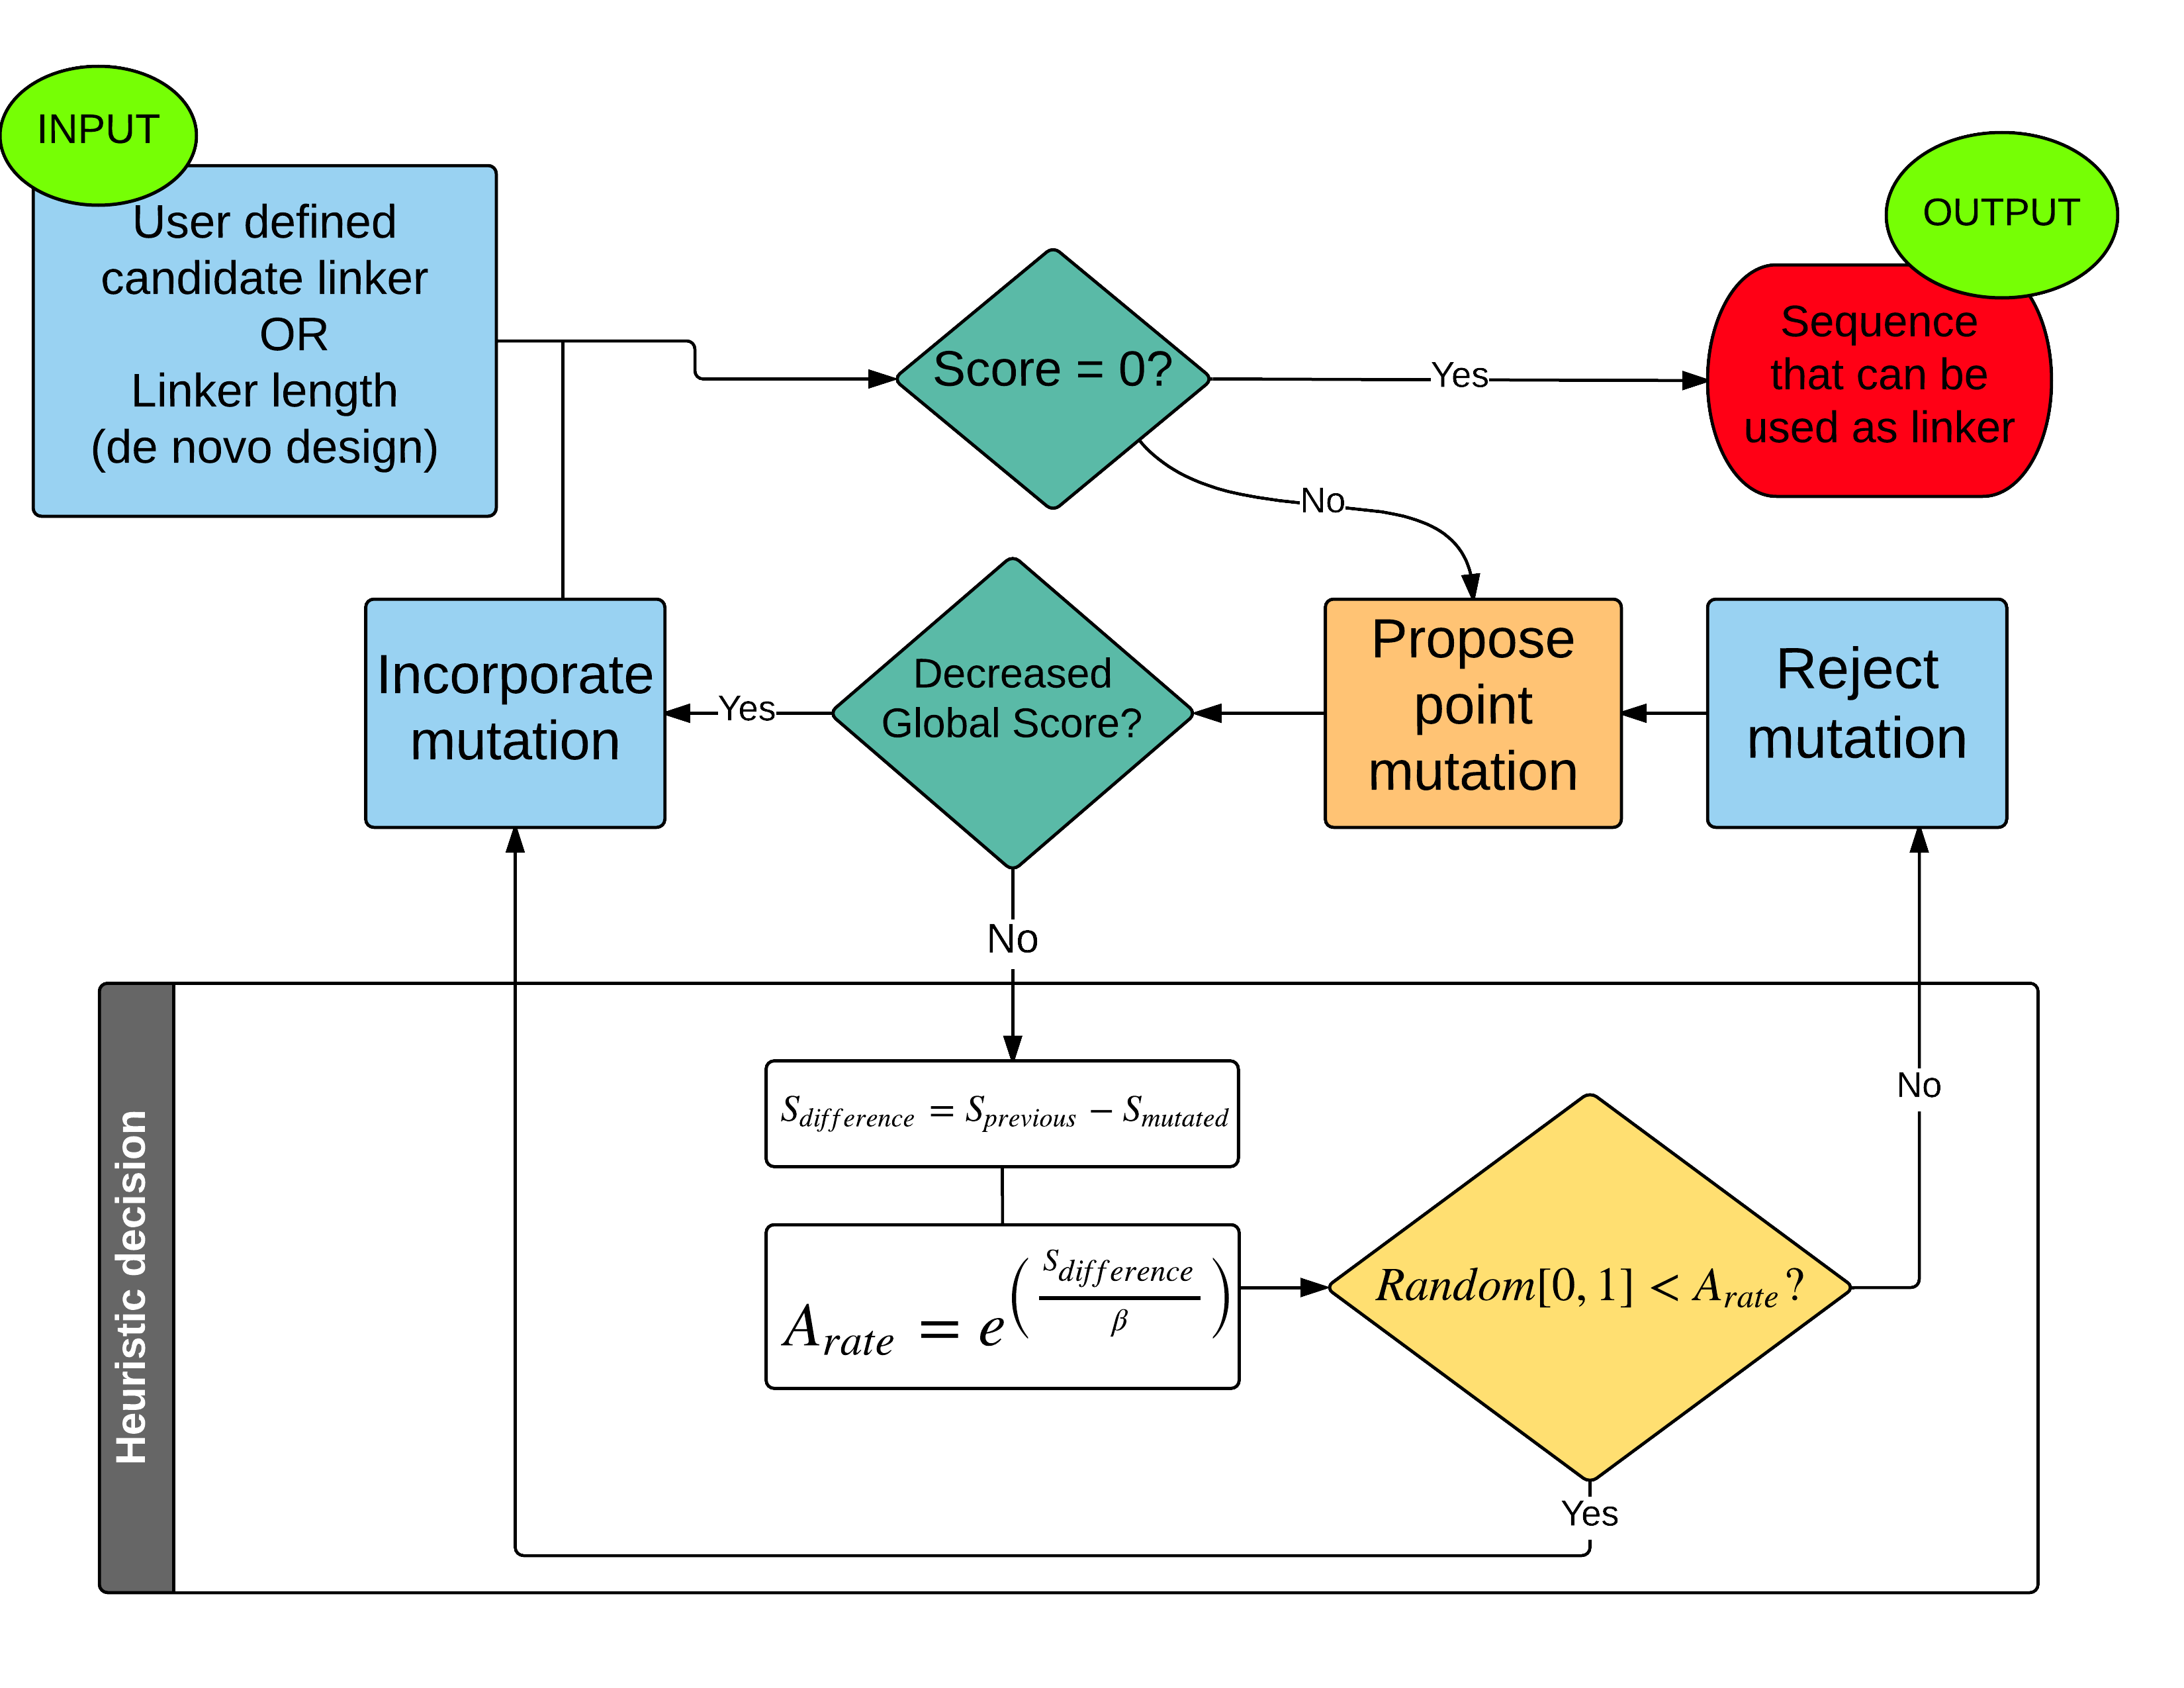
\includegraphics[width=0.99\linewidth, height=230px]{figures/patenaFull.png}
\end{minipage}
\begin{minipage}{0.49\linewidth}
 % \headerbox{Scoring function}{name=scoring,column=1,span=1}{
Sequences are evaluated for structured regions using the algorithms IUPRED\cite{dosztanyi2005pairwise}, ANCHOR\cite{meszaros2009prediction}, TANGO\cite{fernandez2004prediction}, PASTA\cite{trovato2006insight}
and WALTZ\cite{maurer2010exploring}. Putative functional sites are searched using BLAST\cite{altschul1990basic} and sequence patterns in the ELM\cite{puntervoll2003elm} and
PROSITE\cite{sigrist2002prosite} databases. Net charge and UV absorption can also be evaluated at the user's request. Undesired
structure and functional features are mapped to each sequence position, and the total number of undesired
features is calculated, resulting in a global score. For example: 

\vspace{10px}
\hspace{1.4em}
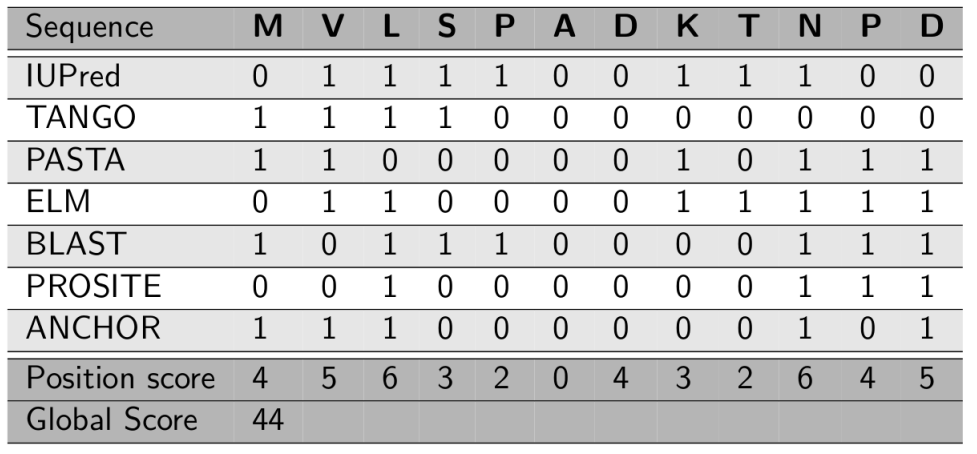
\includegraphics[width=0.89\linewidth, height=115px]{figures/tabla.png}
% \vspace{\vfill}
% \begin{tabular}{llllllllllllll} 
% \hline
% \rowcolor{GrayOscuro}Sequence & \textbf{M} & \textbf{V} & \textbf{L} & \textbf{S} & \textbf{P} & \textbf{A} & \textbf{D} & \textbf{K} & \textbf{T} & \textbf{N} & \textbf{P} & \textbf{D} \\ \hline \hline
%  
% % Puntaje Inicial & 0 & 0 & 0 & 0 & 0 & 0 & 0 & 0 & 0 & 0 & 0 & 0\\ \hline
% \rowcolor{Gray}IUPred           	& 0 & 1 & 1 & 1 & 1 & 0 & 0 & 1 & 1 & 1 & 0 & 0\\ \hline  
% TANGO 		       			& 1 & 1 & 1 & 1 & 0 & 0 & 0 & 0 & 0 & 0 & 0 & 0\\ \hline  
% \rowcolor{Gray}PASTA			& 1 & 1 & 0 & 0 & 0 & 0 & 0 & 1 & 0 & 1 & 1 & 1\\ \hline  
% ELM          	      			& 0 & 1 & 1 & 0 & 0 & 0 & 0 & 1 & 1 & 1 & 1 & 1\\ \hline 
% \rowcolor{Gray}BLAST			& 1 & 0 & 1 & 1 & 1 & 0 & 0 & 0 & 0 & 1 & 1 & 1\\ \hline 
% PROSITE 	      			& 0 & 0 & 1 & 0 & 0 & 0 & 0 & 0 & 0 & 1 & 1 & 1\\ \hline 
% \rowcolor{Gray}ANCHOR	        	& 1 & 1 & 1 & 0 & 0 & 0 & 0 & 0 & 0 & 1 & 0 & 1\\ \hline \hline
% \rowcolor{GrayOscuro}Position score     & 4 & 5 & 6 & 3 & 2 & 0 & 4 & 3 & 2 & 6 & 4 & 5\\ \hline
% \rowcolor{GrayOscuro}Global Score  & 44 &&&&&&&&&&& \\ \hline
% \end{tabular}
\end{minipage}
\end{minipage}
}








\headerbox{Execution time}{name=beta,column=0,span=1,below=method}
{
\begin{center}
%   \begin{minipage}{0.3\linewidth}
% %   \includegraphics[width=\linewidth]{basis-giraffe-example-frame}\\[1em]
  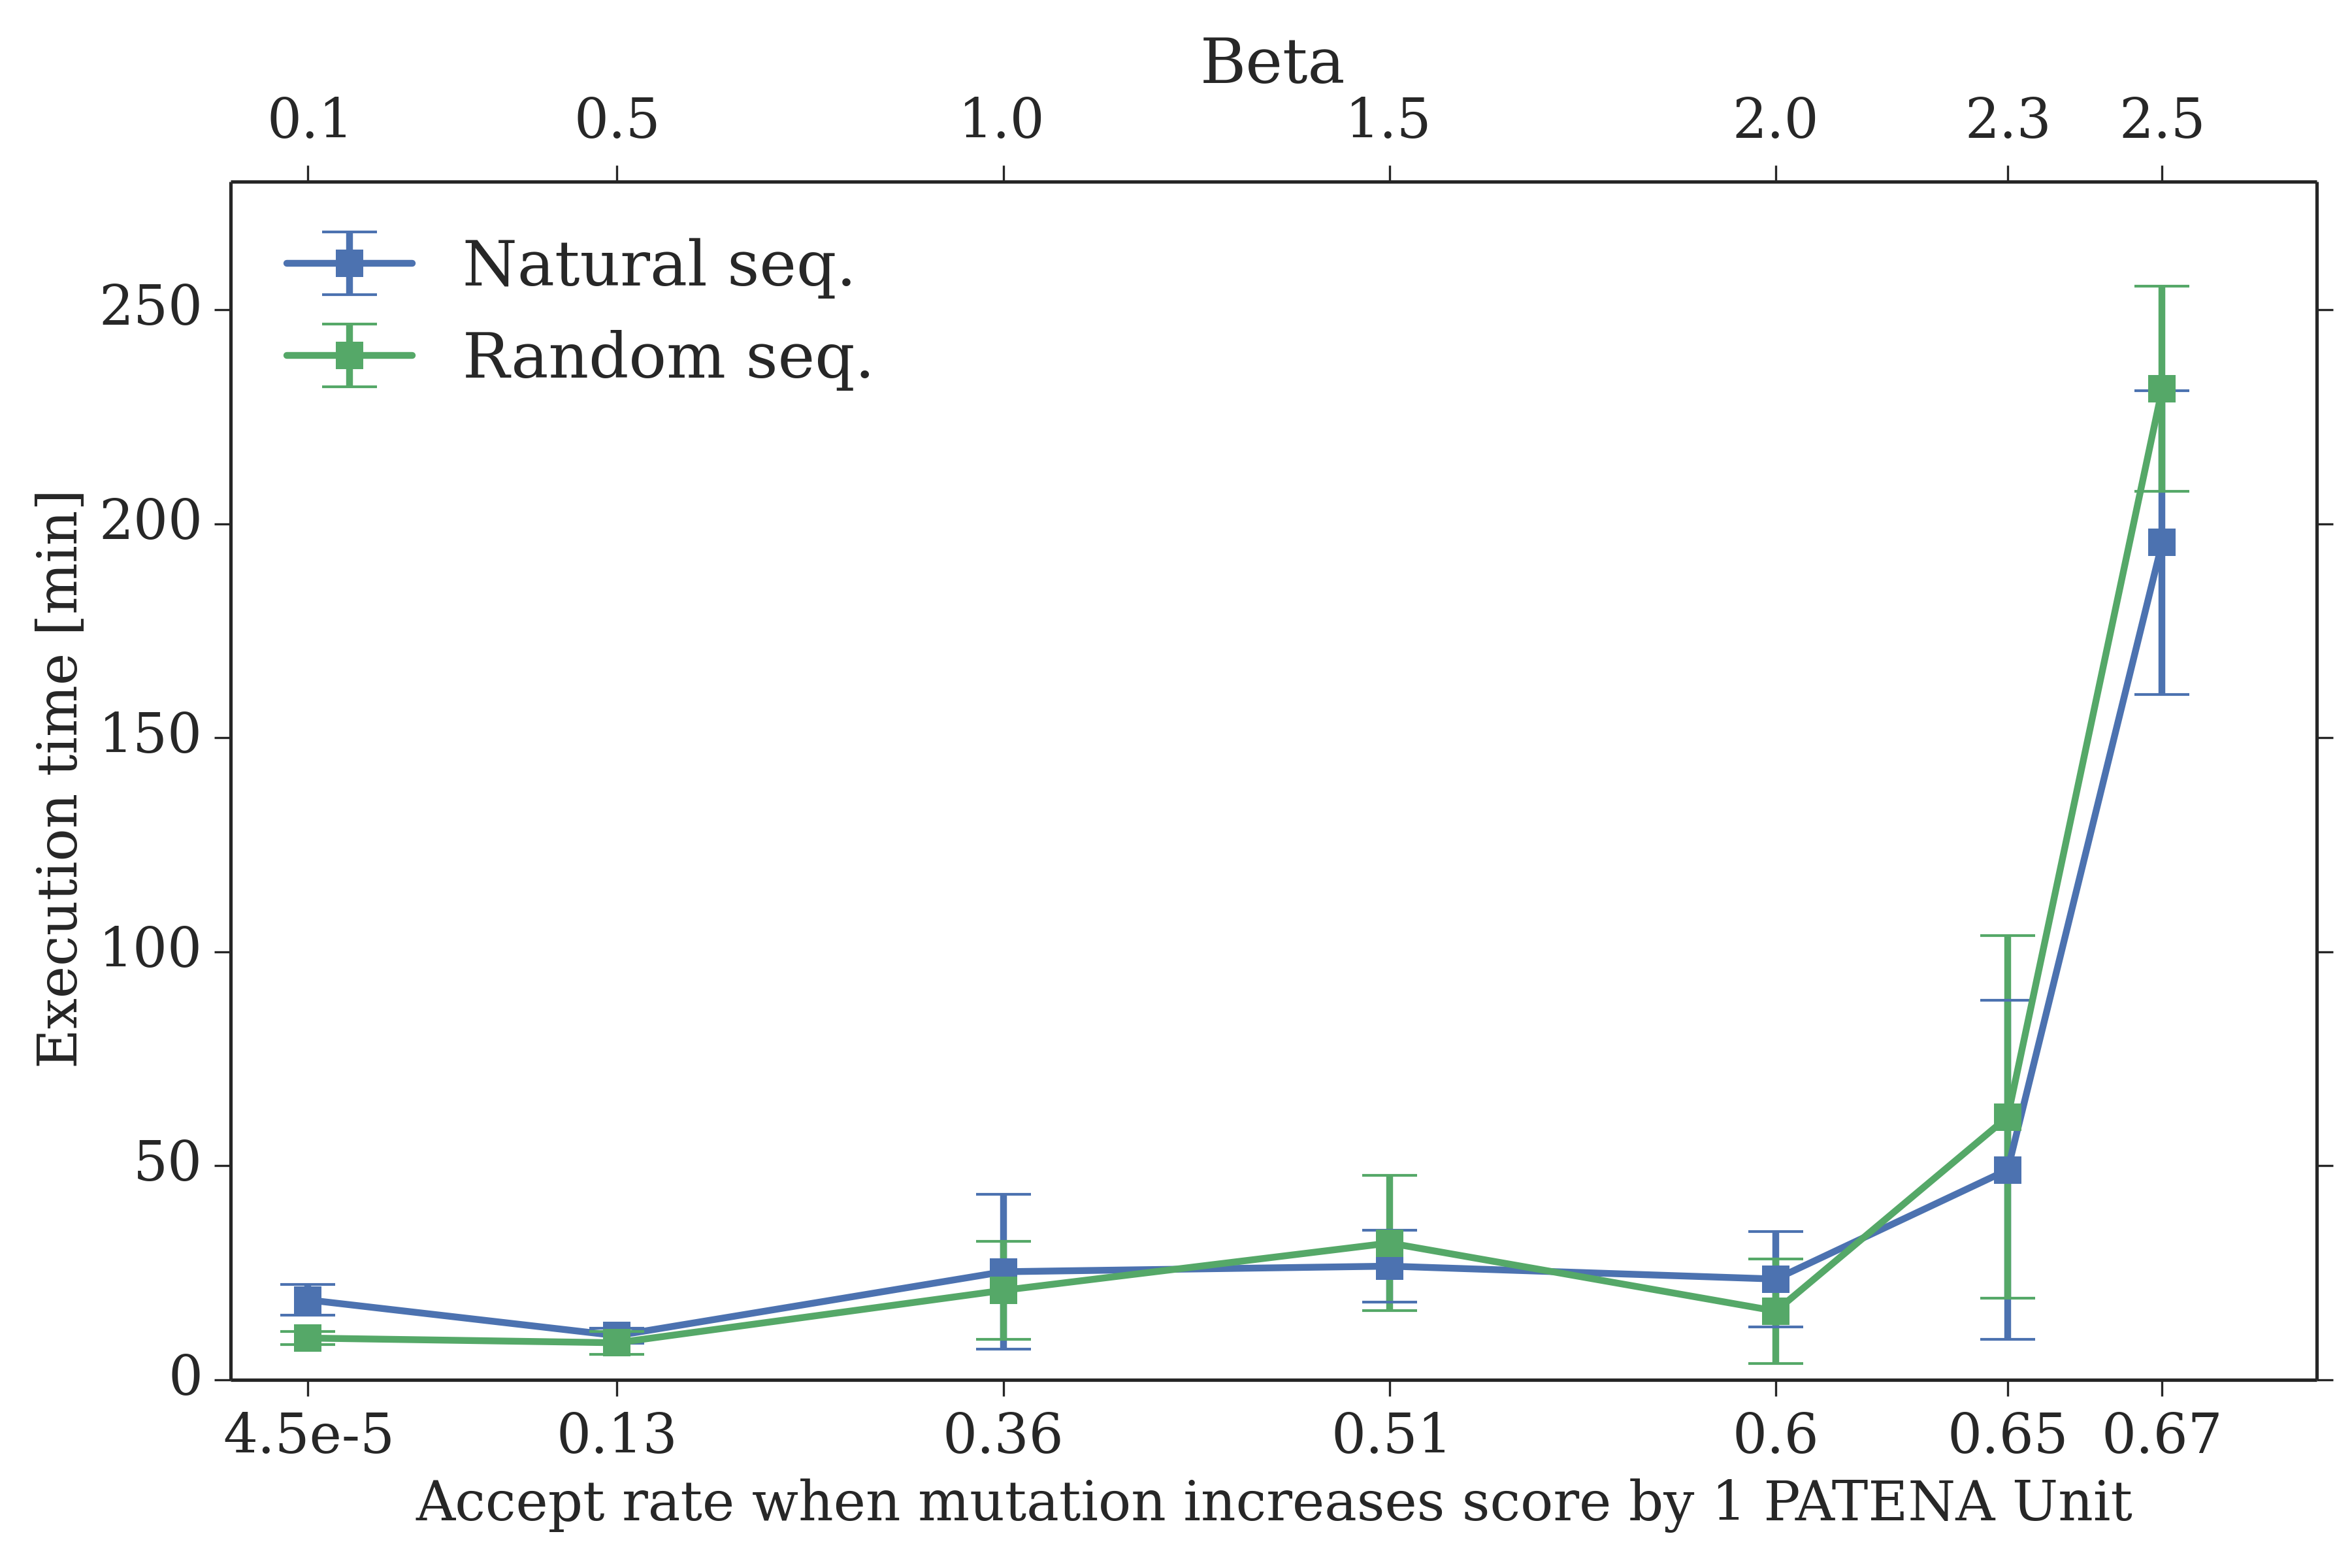
\includegraphics[width=\linewidth]{figures/beta-vs-time-length50-300dpi.png}
% \caption{aaaa}
%   \end{minipage}
  \captionof{figure}{Effective Beta range: Execution times were evaluated for Beta values ranging from 0.1 to 2.5, using random (n=3) and natural (n=3) starting sequences of length 50. \textbf{We choose a Beta value of 1.0 for PATENA.}}
  \label{fig:name}
\end{center}
% Aca va el texto que describe la figura \ref{fig:name}
\begin{center}
%   \begin{minipage}{0.3\linewidth}
% %   \includegraphics[width=\linewidth]{basis-giraffe-example-frame}\\[1em]
%   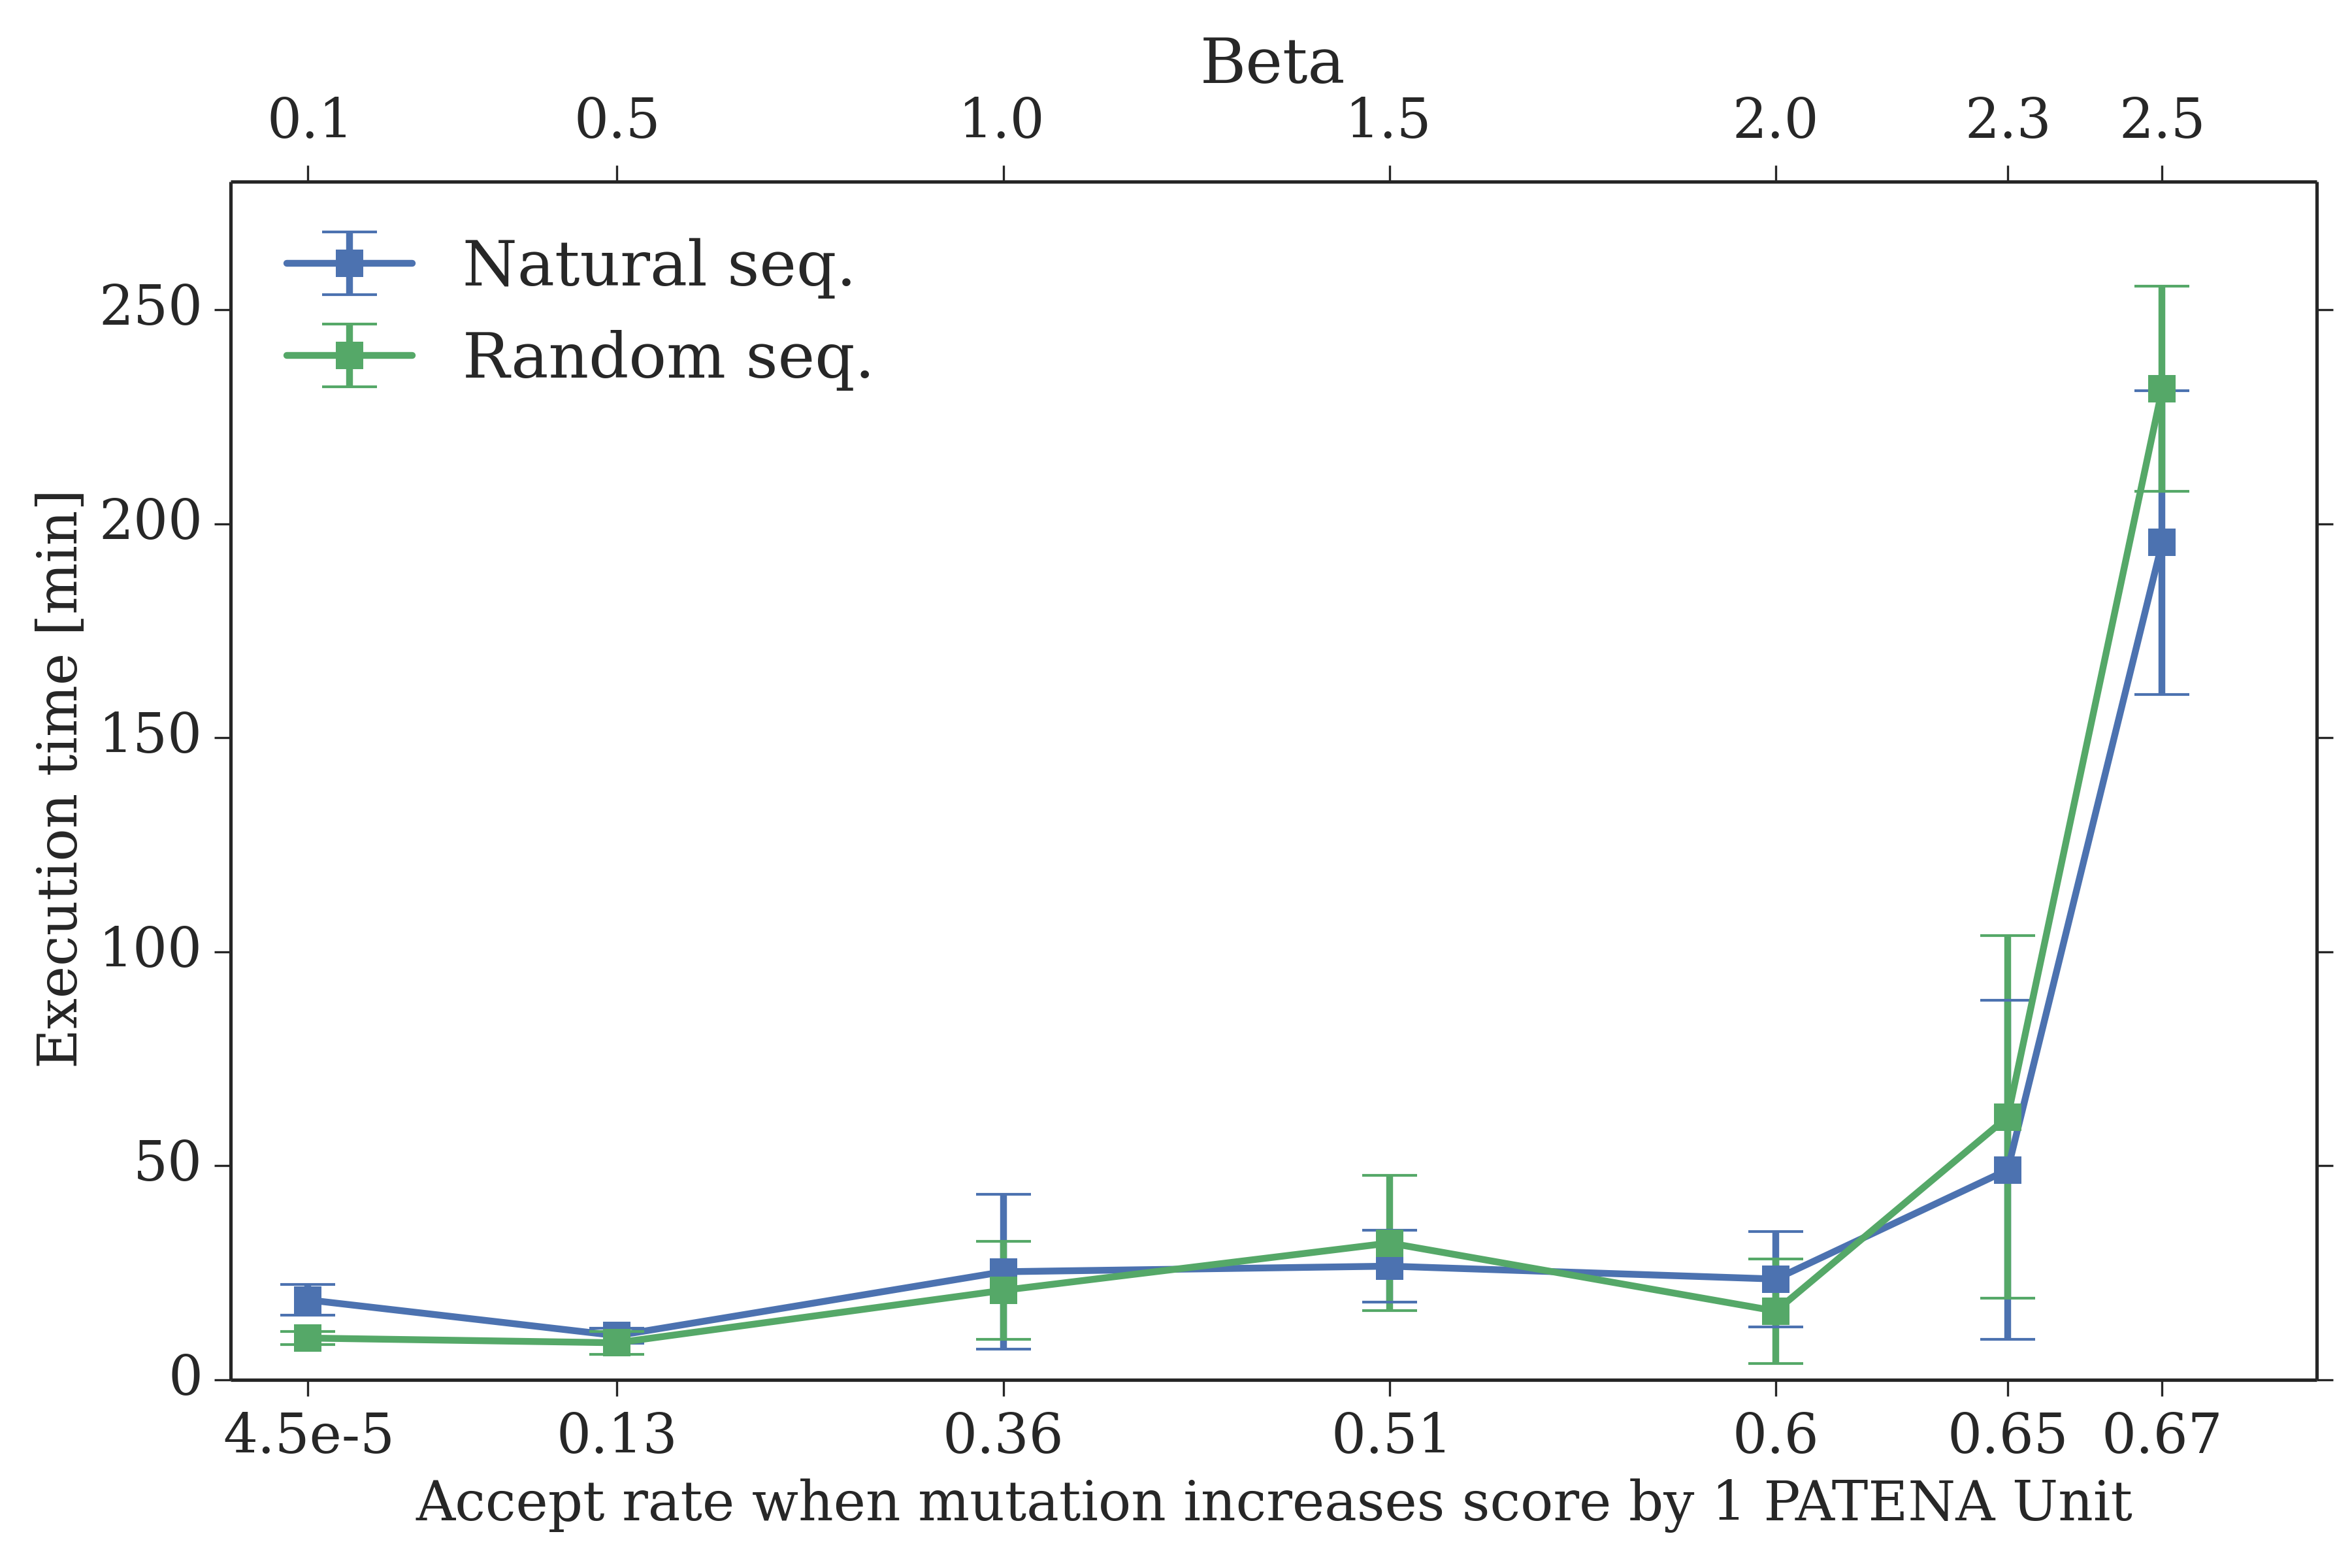
\includegraphics[width=0.5\linewidth]{figures/beta-vs-time-length50-300dpi.png}
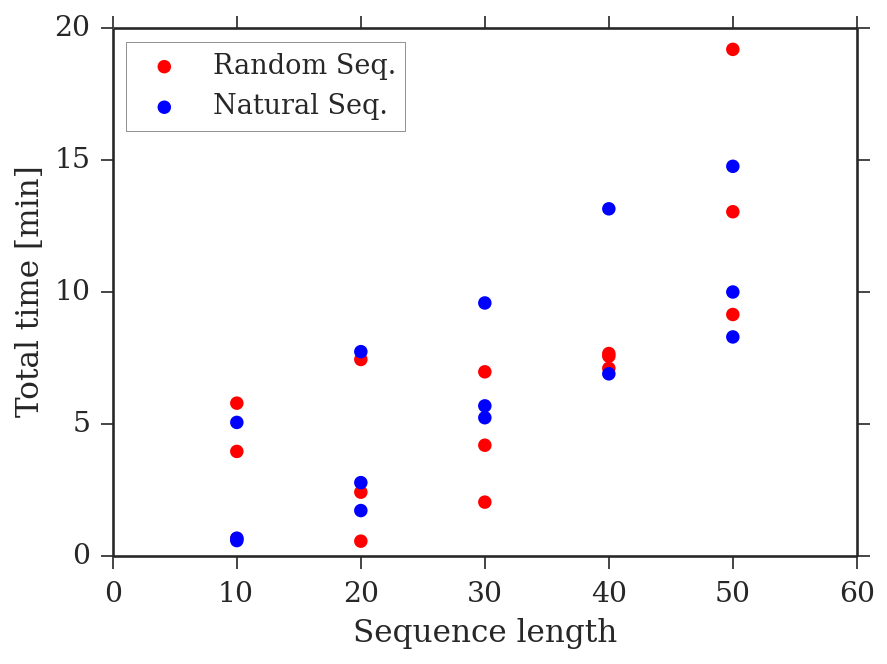
\includegraphics[width=\linewidth, height=150px]{figures/lengthVsTime.png}
 \captionof{figure}{Dependence with length: Evaluation of execution time for a set of 36 random and natural sequences of different lengths. Beta=1.0 \textbf{. The execution time increases with
sequence length in an approximately linear manner.}}
  \label{fig:name2}
\end{center}

}





\headerbox{Resulting designs}{name=divergence,column=1,span=2,below=method}
{
These results were obtained using Beta = 1.0. Aminoacid composition in the UniProtKB/Swiss-Prot data bank was used to propose mutations.\\
% was chosen as default for PATENA.\\
% \begin{flalign*}
%   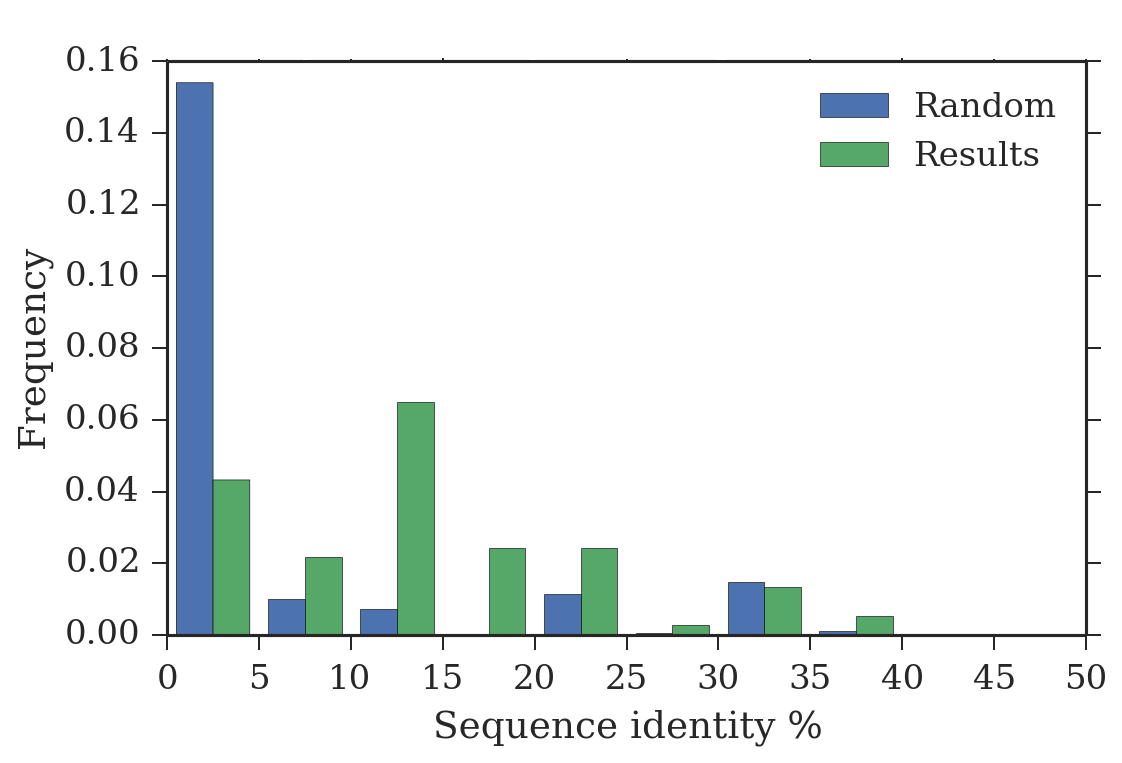
\includegraphics[width=0.4\linewidth,left]{figures/againstInitial-random.png}
% \end{flalign*}
\hspace{-15px}
  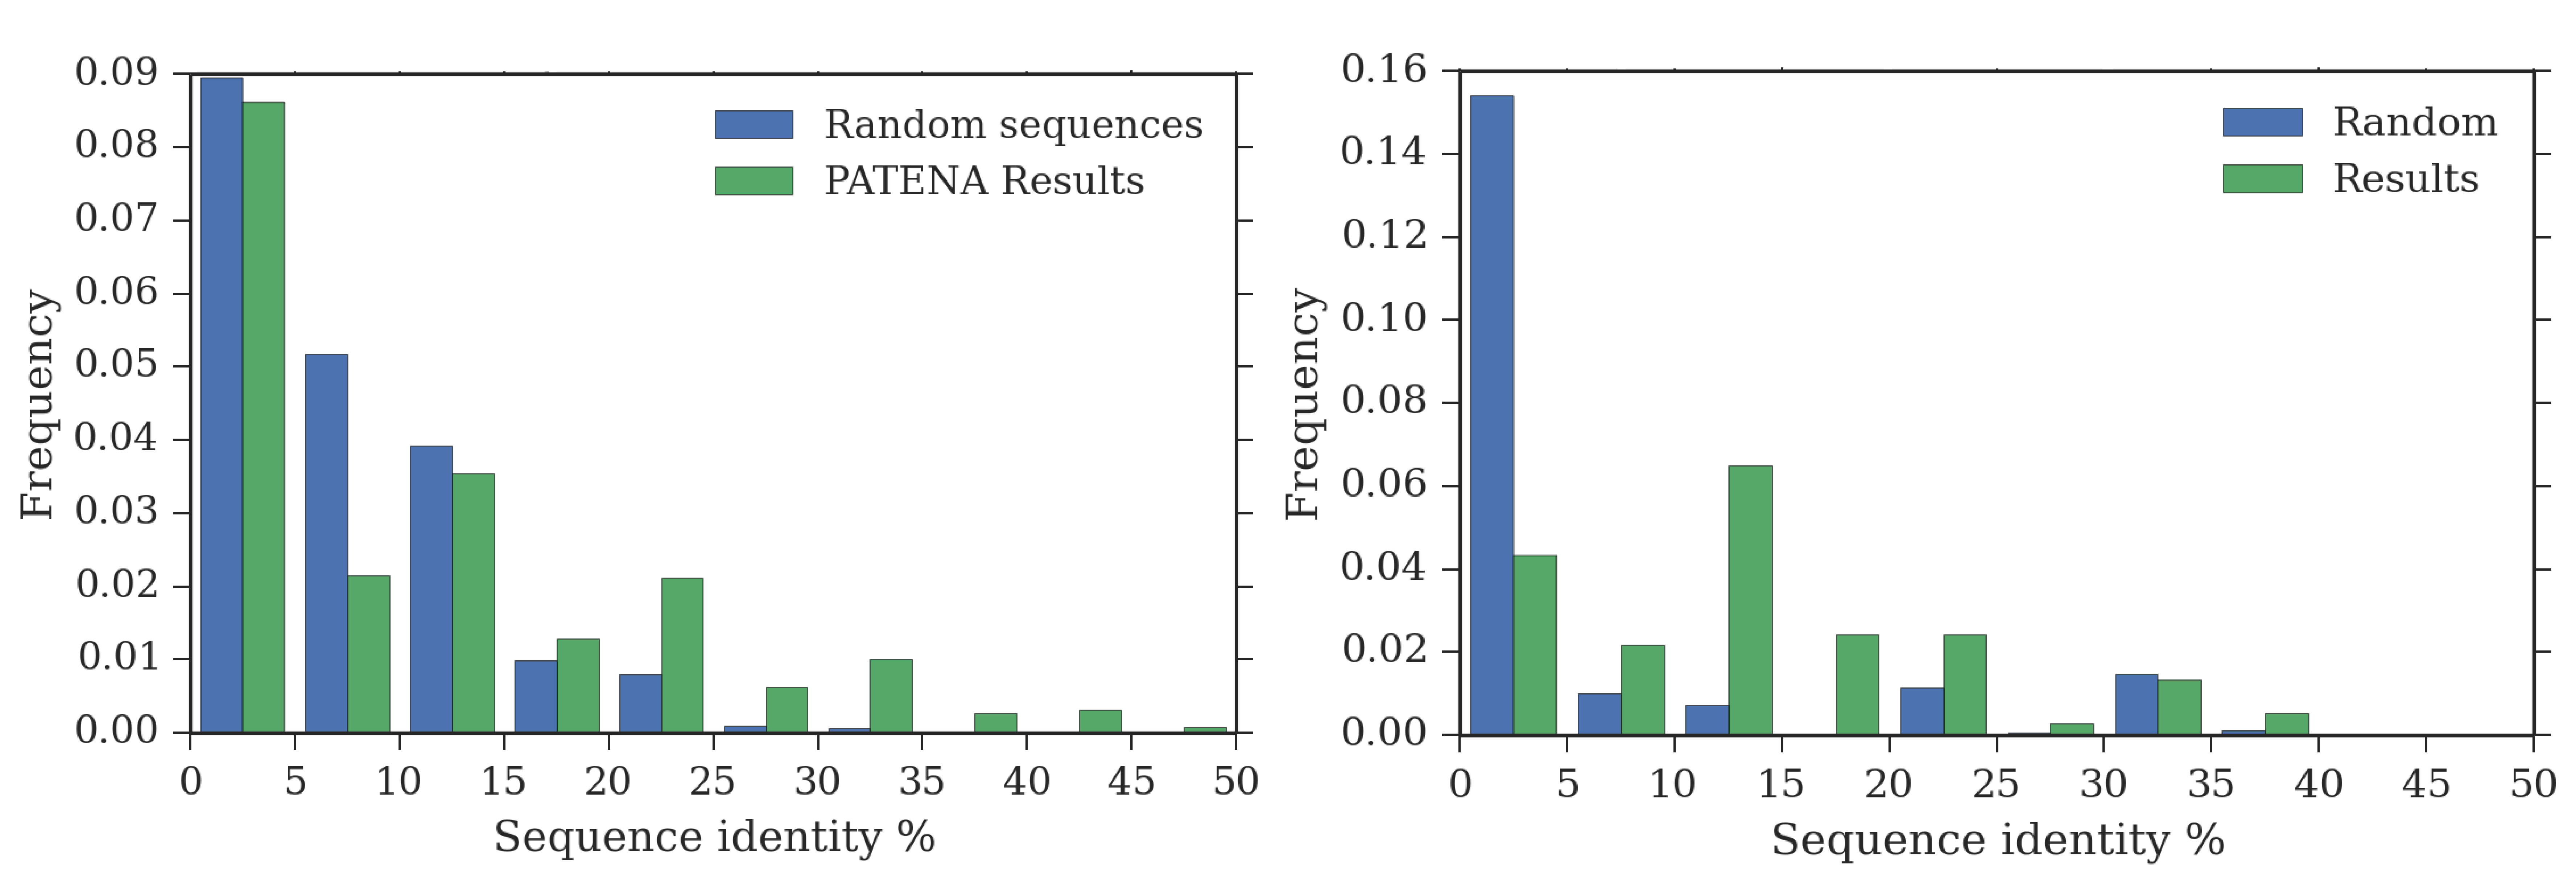
\includegraphics[width=\linewidth,height=148px]{figures/dosJuntas.png}
 \captionof{figure}{Divergence evaluation: 74 different designs were obtained starting from a unique sequence. Figures shows identity against initial sequence (left) and between results(right).
\textbf{Results form a heterogeneous set. Despite having a high number of mutations, resulting sequences still maintain certain similarity with initial sequence.}}
% mayor que random pero claramente hubo bastantes mutaciones(contra inicial)
% mayor que random pero claramente heterogeneas(entre resultados)
 % \vspace{10px}
%   \hspace{-15px}
%  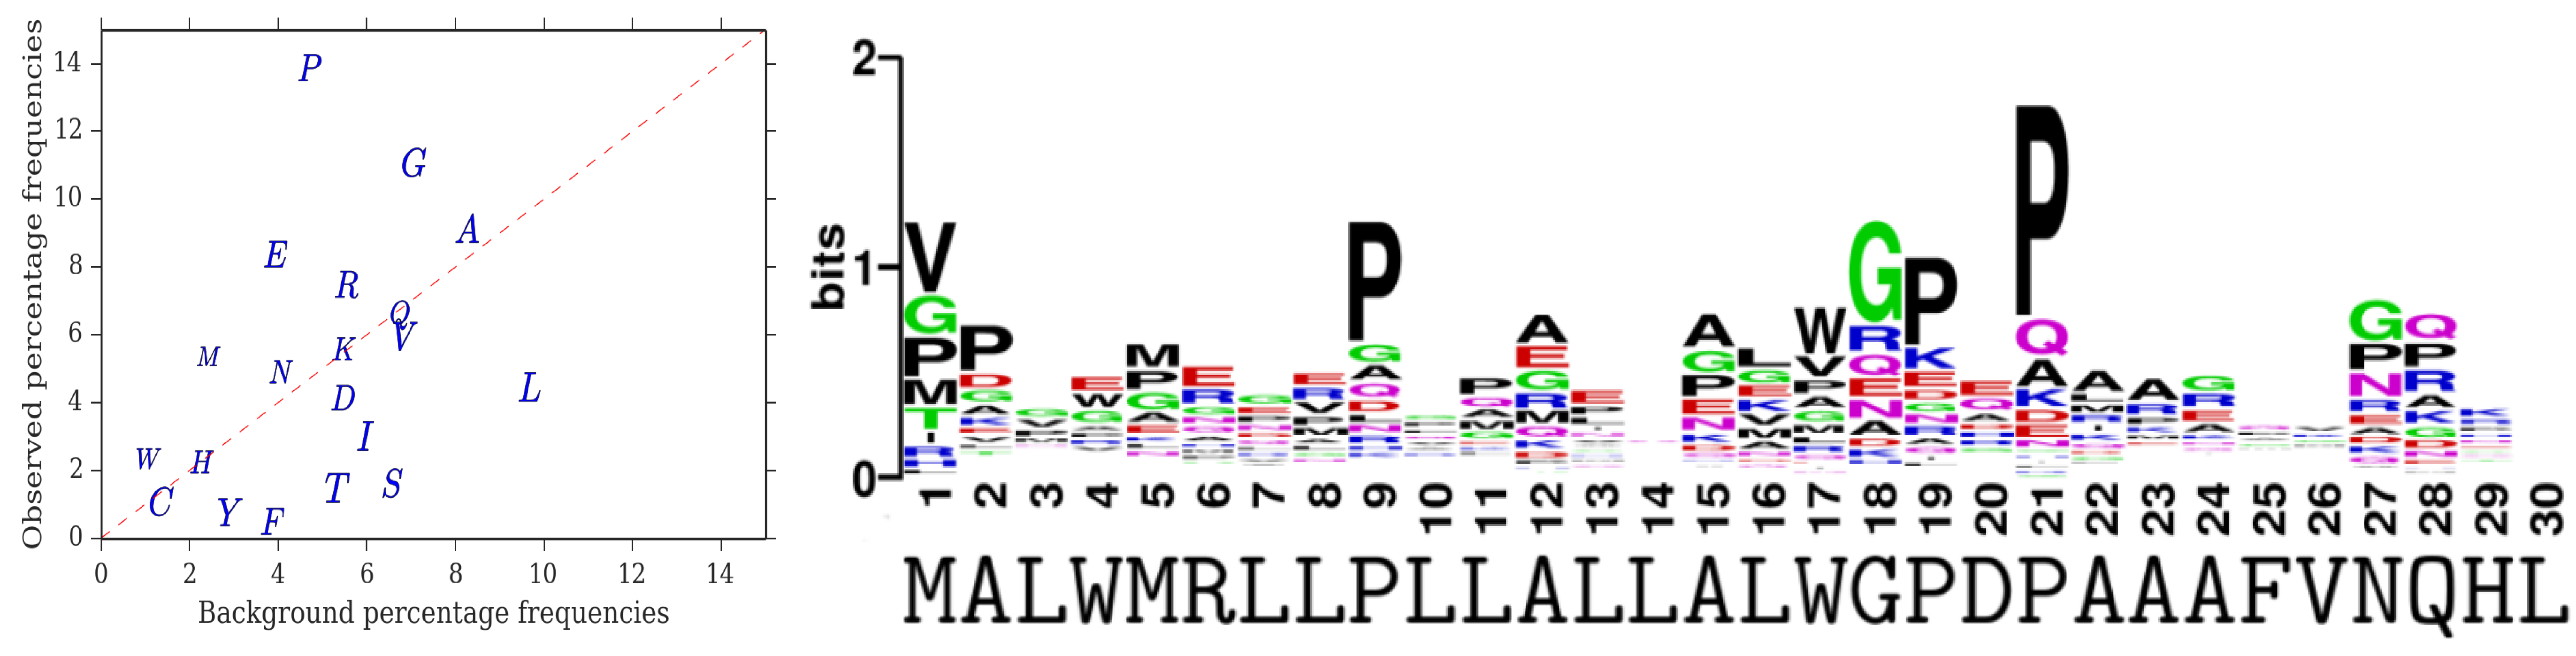
\includegraphics[width=\linewidth]{figures/doblete.png}
%  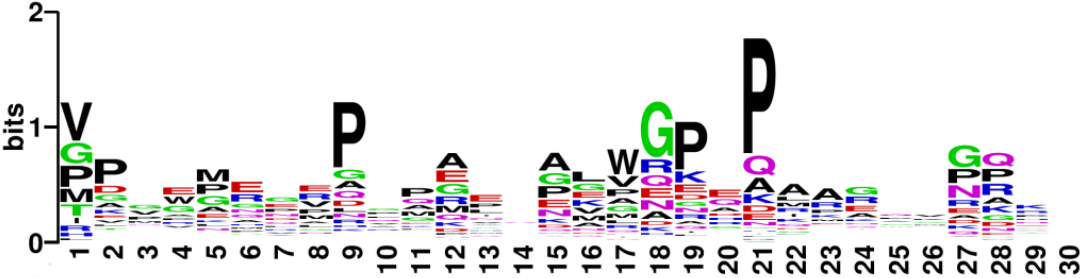
\includegraphics[width=\linewidth]{figures/logo.png}
% \hspace{23px} 
\includegraphics[width=0.95\linewidth]{figures/sequence.png}
% 
\begin{figure}[H]
  \centering
  \begin{minipage}[b]{0.56\textwidth}
    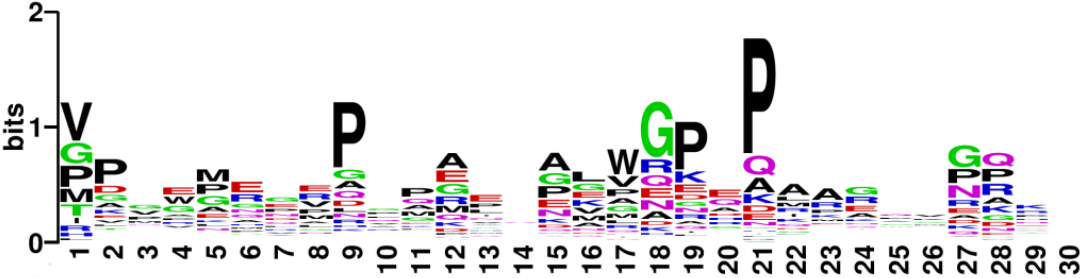
\includegraphics[width=0.98\textwidth,height=120px]{figures/logo.png}
   
    \hspace{14px} 
\includegraphics[width=0.92\linewidth]{figures/sequence.png}
\captionof{figure}{Sequence logo obtained from the set of 74 different designs. The starting sequence is shown under the logo.
\textbf{Most conserved positions are those initially containing small and disorder-favoring(disorder-promoting) residues(G or P)}}
% expected to keep a flexible(G) and disordered conformation(P)}}
%     \caption{Flower one.}
% \captionof{figure}{S}
  \end{minipage}
  \hfill
  \begin{minipage}[b]{0.42\textwidth}
    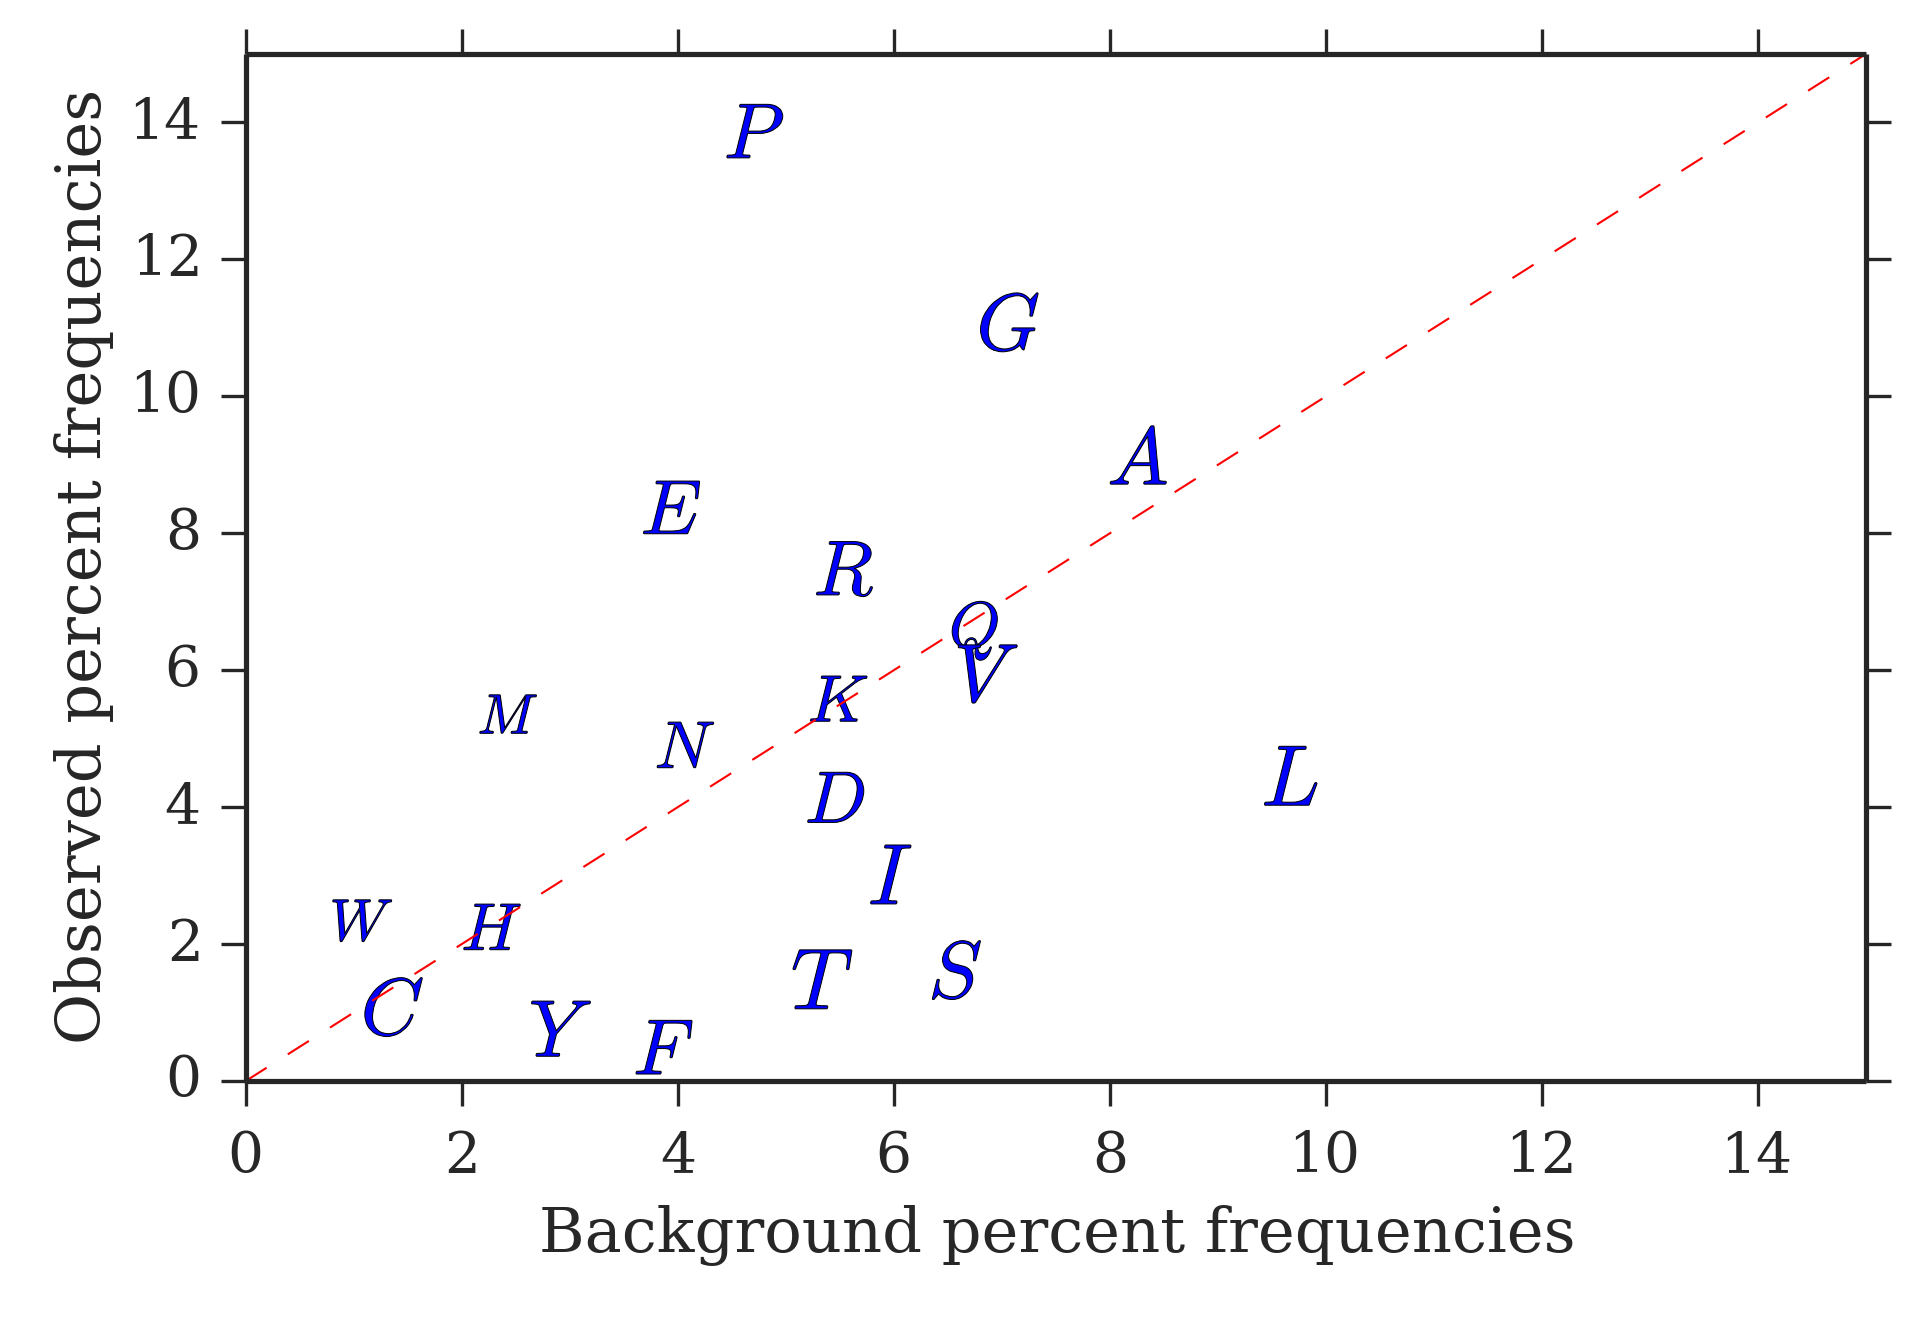
\includegraphics[width=\textwidth, height=135px]{figures/frequenciesComparison.png}
    \captionof{figure}{Comparison of frequencies imposed during mutation attempts and frequencies observed in resulting set. \textbf{Observed frequencies don't deviate from background. Highest variation is found in Proline frequence, a disorder-promoting amino acid.}}
%     \caption{Flower two.}
  \end{minipage}
\end{figure}



% \begin{figure}[H]
%   \begin{subfigure}[b]{0.4\textwidth}
%     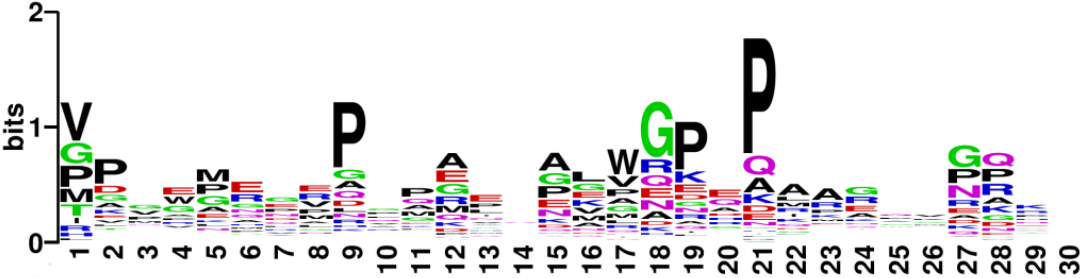
\includegraphics[width=1.4\textwidth]{figures/logo.png}
%     \caption{Flower one.}
%     \label{fig:f1}
%   \end{subfigure}
%   \hfill
%   \begin{subfigure}[b]{0.4\textwidth}
%     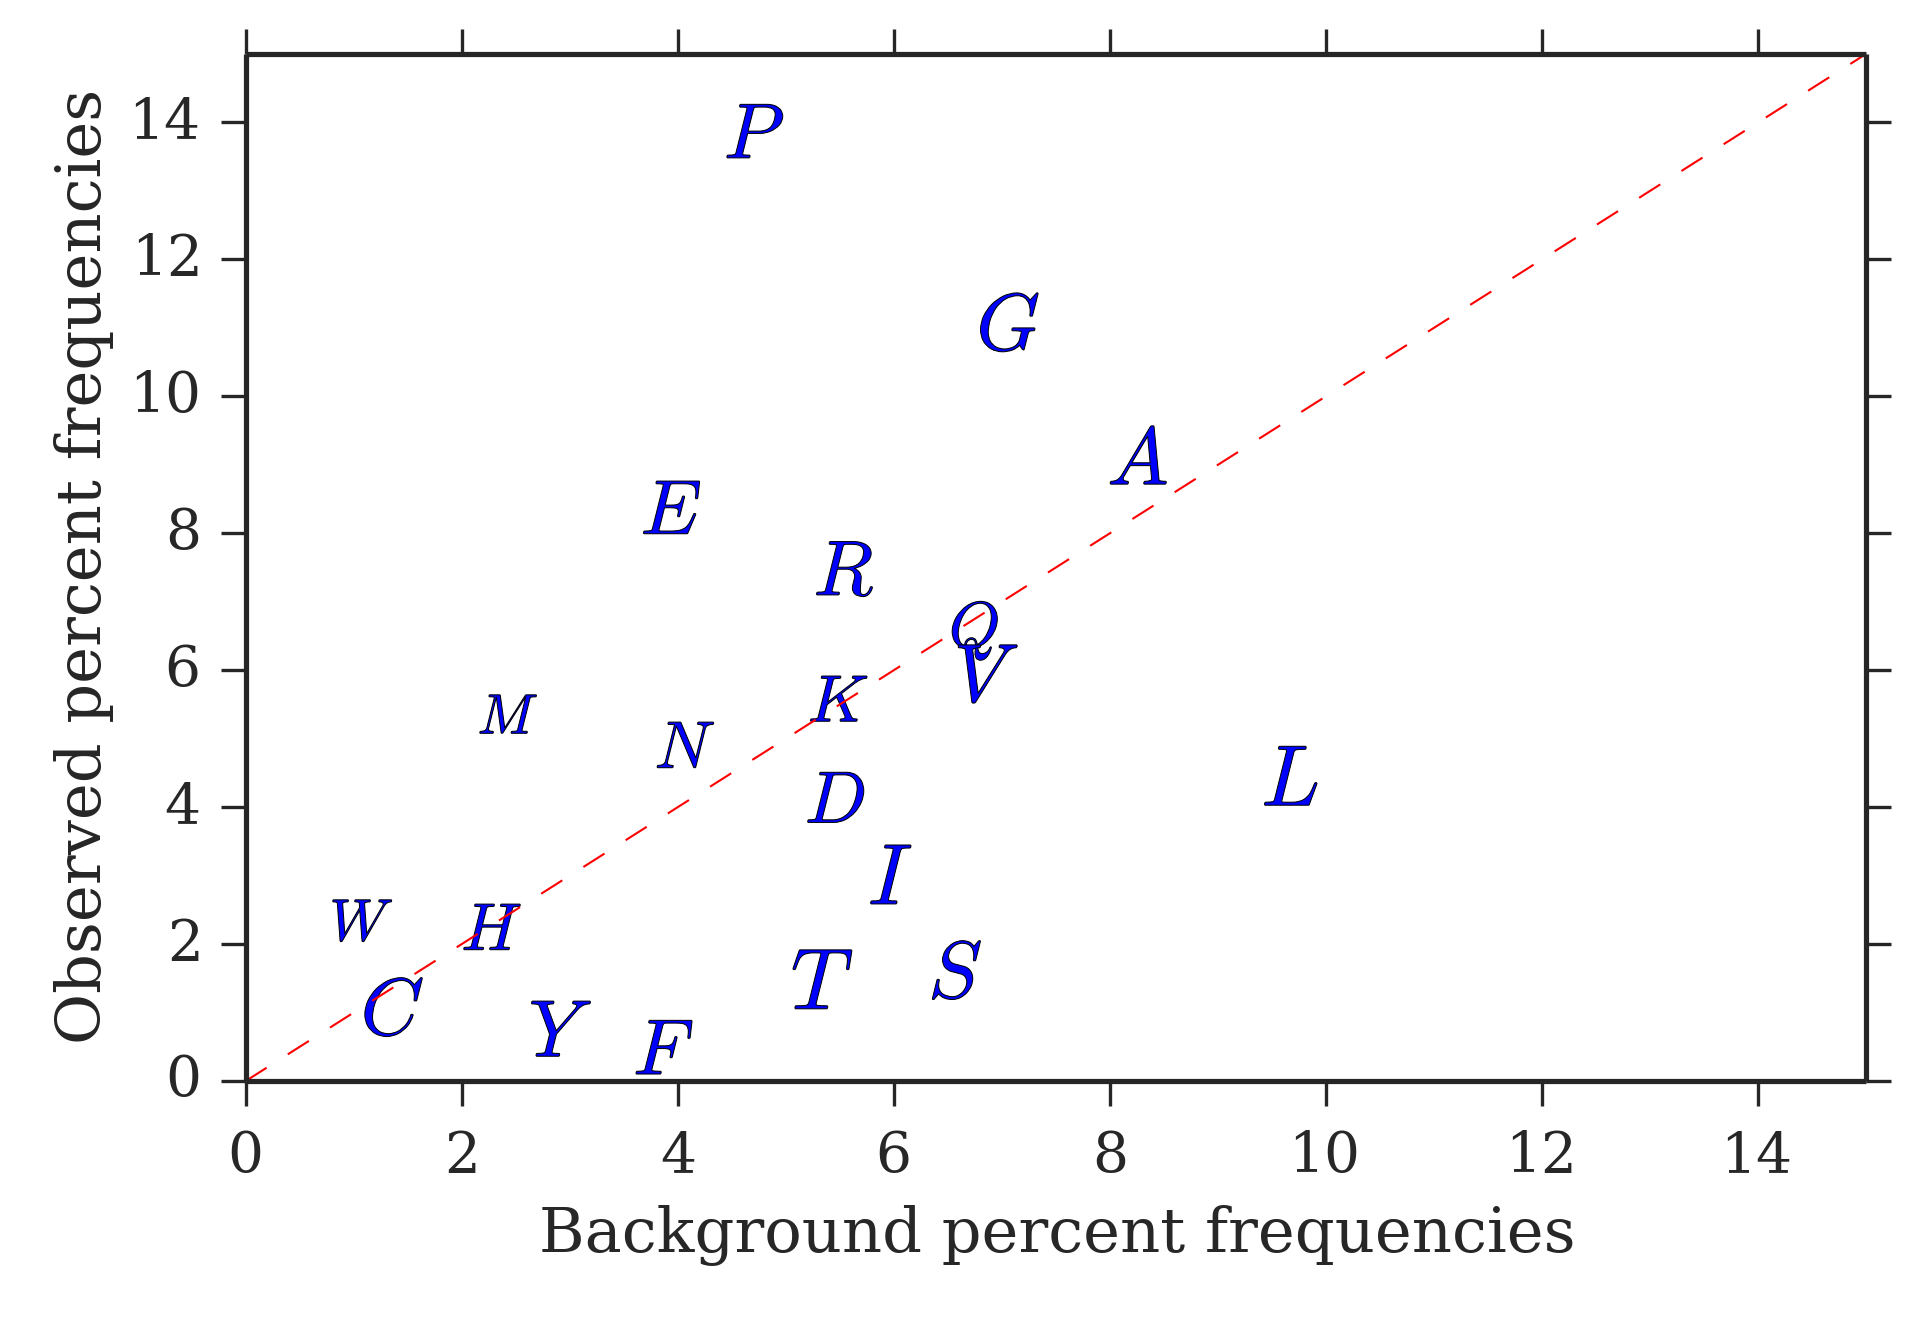
\includegraphics[width=\textwidth]{figures/frequenciesComparison.png}
%     \caption{Flower two.}
%     \label{fig:f2}
%   \end{subfigure}
%   \caption{My flowers.}
% \end{figure}




}



%%%%%%%%%%%%%%%%%%%%%%%%%%%%%%%%%%%%%%%%%%%%%%%%%%%%%%%%%%%%%%%%%%%%%%%%%%%%%%
\headerbox{References}{name=references,column=2,span=1,below=divergence}{
%%%%%%%%%%%%%%%%%%%%%%%%%%%%%%%%%%%%%%%%%%%%%%%%%%%%%%%%%%%%%%%%%%%%%%%%%%%%%%
\footnotesize % Make the whole text smaller
\vspace{-0.4em} % Save some space at the beginning
% \bibliographystyle{plain}							% Use plain style
% \printbibliography
\setlength\bibitemsep{2pt}
\renewcommand*{\bibfont}{\tiny}
\renewcommand{\section}[2]{\vskip 0.05em}		% Omit "References" title
% \begin{thebibliography}{1}							% Simple bibliography with widest label of 1
% \itemsep=-0.01em										% Save space between the separation
% \setlength{\baselineskip}{0.4em}					% Save space with longer lines
% % \bibitem{prevWork1} Laszlo Gulyas, Richard Legendi: \emph{Effects of Sample Duration on Network Statistics in Elementary Models of Dynamic Networks}, International Conference on Computational Science, Singapore (2011) 
% % \bibitem{prevWork2} Laszlo Gulyas, Susan Khor, Richard Legendi and George Kampis \emph{Cumulative Properties of Elementary Dynamic Networks}, The International Sunbelt Social Network Conference XXXI (2011)
% % \bibitem{gulya-kampis1} Gulyas, Laszlo et al.: \emph{Betweenness Centrality Dynamics in Networks of Changing Density}. Presented at the 19th International Symposium on Mathematical Theory of Networks and Systems (MTNS 2010)
% \end{thebibliography}
\printbibliography[title='']
}


%%%%%%%%%%%%%%%%%%%%%%%%%%%%%%%%%%%%%%%%%%%%%%%%%%%%%%%%%%%%%%%%%%%%%%%%%%%%%%
  \headerbox{Conclusions}{name=conclusions,column=0,span=2,below=beta}{
%%%%%%%%%%%%%%%%%%%%%%%%%%%%%%%%%%%%%%%%%%%%%%%%%%%%%%%%%%%%%%%%%%%%%%%%%%%%%%
%   Conclusiones!!!!
  \begin{itemize}
 \item PATENA can find suitable protein linkers in a short execution time.
 \item The set of designs that can be obtained from the same sequence shows high diversity. 
 \item Allows for development of server to design linker sequences.
%  \item We interpret that the space of suitable linker sequences is a large fraction of the whole sequence space.
\end{itemize}
}

\end{poster}

\end{document}

